%%
%% Capítulo 1: Modelo e Descrição Geral para quem usa o LaTeX
%%
\chapter{Fundamentação Teórica}
\label{Cap:fundamentacao}

Neste capítulo tem-se como objetivo apresentar conceitos e fundamentos relacionados as áreas de segurança computacional e inteligência artificial, as quais são de interesse primordial para o presente trabalho.

Na seção de segurança computacional, são citados alguns dos tipos de ameaças existentes, definição e conceitos da linha de pesquisa de detecção de intrusão, assim como os sistemas de detecção de intrusão (SDI) e suas principais características arquiteturais.

A seção de inteligência artificial apresenta contextualização acerca de temas como aprendizado de máquina, aprendizado supervisionado, tipos de modelos e seus paradigmas, tal como métricas geralmente utilizadas para avaliação dos modelos construídos.

\section{Segurança Computacional}
\label{Sec:seguranca-computacional}
A exposição de grande volume de informação em uma velocidade, até poucos anos atrás, inimaginável é uma consequência da popularidade de Internet e da facilidade de acesso à mesma, após a chegada de dispositivos móveis, computadores pessoais, televisores inteligentes, entre outros.

De mesmo modo que este fenômeno foi responsável por vários avanços tecnológicos benéficos a sociedade, foi também responsável pelo crescimento drástico de ocorrências de atividades ilícitas no mundo digital, visto que todo sistema de informação ou infraestrutura computacional pode estar sujeito a apresentar vulnerabilidades.

Para identificar e auxiliar em medidas a serem tomadas, diante do acontecimento de eventos maliciosos em ambiente computacional, a área de pesquisa denominada ``Segurança Computacional`` foi criada e está em constante aprimoramento por meio de pesquisas científicas. Embora a amplitude de temas abordados dentro da área de segurança seja enorme, \citeasnoun{gollmann2010} divide a mesma em quatro partes, de acordo com diferentes interesses:

\begin{itemize}
    \item Controle de acesso a um sistema;
    \item Controle de acesso a recursos gerenciados por um sistema;
    \item Proteção de dados transmitidos entre sistemas;
    \item Proteção de sistemas contra \textit{inputs} maliciosos.
\end{itemize}

Cada um dos tópicos citados e discutidos por \citeasnoun{gollmann2010} tem suma importância no que se refere a segurança computacional, pois englobam praticamente todos os focos de incidentes no mundo digital. O presente trabalho, por sua vez, encontra-se enquadrado no tópico de "proteção de dados sendo transmitidos entre sistemas", visto que são levados em conta principalmente eventos ocorridos durante a comunicação de computadores por meio de redes de computadores, ou seja, mediante análise de tráfego de dados.

\begin{comment}
\subsection{Tipos de Ameaças}
\label{Sec:subsecoes}

Tipos de ataques interessantes de abordar:
DoS (Comentar que podem ser utilizadas várias ferramentas: HULK, GoldenEye, Slowloris)
Brute Force (Citando Patator, que oferece suporte pra vários serviços, mas focar em SSH e FTP que estão presentes na CICIDS2017)
PortScan
Botnet
Infiltration (iciss20140_submission_35.pdf downloads)

\end{comment}

\subsection{Detecção de Intrusão}
\label{Sec:figuras}

Eventos intrusivos correspondem àqueles que infringem princípios básicos da segurança computacional, como confidencialidade, integridade, autenticidade e/ou disponibilidade de informações ou recursos. Diante da necessidade e da importância de identificar e analisar esses eventos, delineou-se a área de detecção de intrusão, a qual trata-se da linha de pesquisa responsável pelo desenvolvimento de técnicas que objetivam a identificação de intrusões e atividades maliciosas, a fim de alertar e possibilitar contramedidas aos incidentes ocorridos.

SDI são considerados uma das principais ferramentas utilizadas para esta tarefa, visto que são capazes de combinar diferentes estratégias e características arquiteturais, com o intuito de  identificar comportamentos anômalos que apontem suspeitas de que atividades não lícitas estejam sendo desempenhadas em computadores, sistemas, redes de computadores, entre outros.

Embora diversas classificações de sistemas de detecção de intrusão tenham sido propostas ao longo do tempo, não existe uma taxonomia aceita de forma padronizada e universal, visto que as abordagens possuem prós e contras, acarretando em \textit{tradeoffs} que devem ser avaliados de acordo com o objetivo específico do sistema de detecção de intrusão em questão. Alguns desses aspectos são apresentados a seguir \cite{lazarevic2005}:

\begin{itemize}
    \item \textbf{Fonte de dados:} alguns exempos de fonde dados de SDI são \textit{host} (sistema operacional da máquina local), rede de computadores, logs de aplicações, sensores de alertas.
    \item \textbf{Estratégia de análise:} análise por abuso compreende na técnica mais comumente utilizada, onde o SDI monitora os dados a fim de identificar a ocorrência de comportamentos previamente catalogados, enquanto na análise por anomalia o SDI busca por comportamentos que diferem de atividades definidas e consideradas normais, utilizando diferentes técnicas como regras, métodos estatísticos, cálculo de distâncias, definição de perfis, e outros. Vários SDI também utilizam abordagens híbridas.
    \item \textbf{Frequência de uso:} a análise pode ser realizada tanto em tempo real, monitorando fluxo contínuo de dados, quanto periodicamente, de forma \textit{offline}, investigando lotes de dados, como em auditorias, por exemplo.
    \item \textbf{Arquitetura:} quanto a arquitetura, os SDI podem ser centralizados ou distribuídos. Os SDI centralizados são geralmente utilizados para detectar intrusões feitas em um único sistema a ser monitorado. Com o surgimento de ataques coordenados e distribuídos, com várias máquinas envolvidas, surgiu a necessidade de também monitorar sistemas de forma distribuídas e cooperativa.
    \item \textbf{Tipo de resposta:} SDI podem agir de forma ativa (aplicando contramedidas, como alteração nos serviços disponíveis em um servidor, por exemplo) ou passiva (apenas registrando o comportamento ilícito, eventualmente emitindo alertas) quando uma atividade anômala é identificada.
\end{itemize}

Ainda que não haja consenso na definição de características dos SDI, de modo geral, todos seguem uma estrutura bastante semelhante uns aos outros no que se refere a seus componentes. Na Figura \ref{fig:ids-components} é apresentado um \textit{framework} arquitetural que ilustra os principais componentes que compõem um sistema de detecção de intrusão:

\begin{figure}[!hbt]
\centering 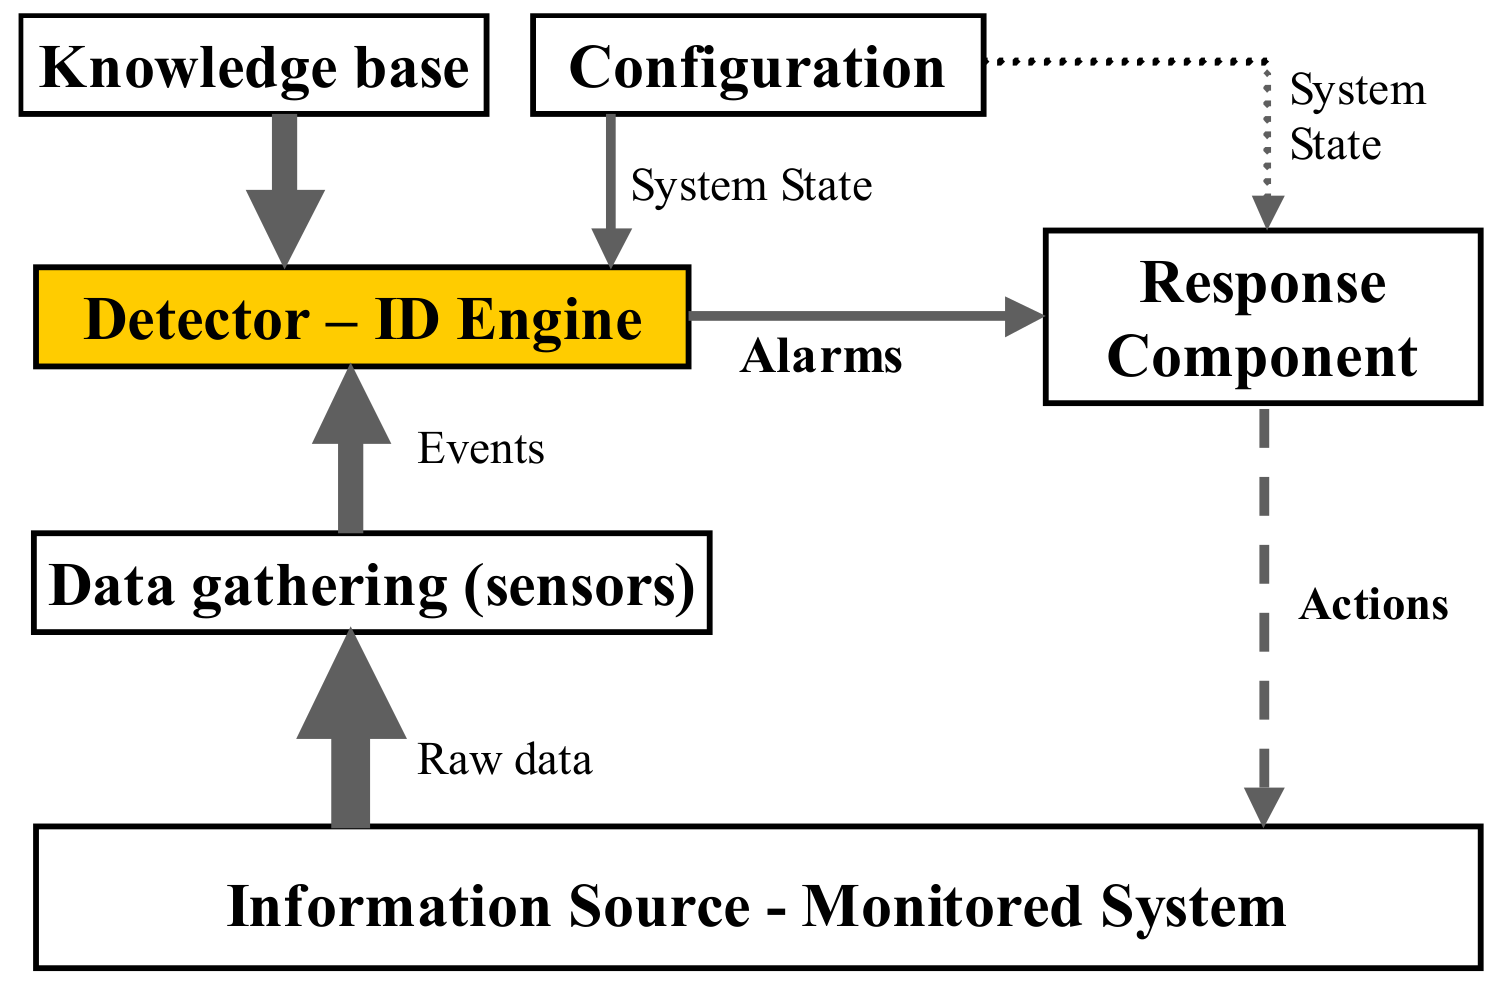
\includegraphics[width=12cm]{{Cap2/ids-components-framework.png}}
\caption{Arquitetura básica de componentes de sistemas de detecção de intrusão (SDI). \cite{lazarevic2005}}
\label{fig:ids-components}
\end{figure}

Conforme apresentado na Figura \ref{fig:ids-components}, os principais componentes são os seguintes:

\begin{itemize}
    \item \textbf{Coletor de dados (\textit{Data gathering device})}: responsável pela coleta de dados do sistema monitorado, mediante geração de \textit{log} e/ou captura e processamento de pacotes de dados, por exemplo.
    \item \textbf{Motor de análise de detecção intrusão (\textit{Detector - Intrusion detection analysis engine}}): componente que processa as informações coletadas para identificar atividades intrusivas.
    \item \textbf{Base de conhecimento (\textit{Knowledge base})}: geralmente contém os dados capturados pelos sensores de coleta, porém de maneira formatada e pré-processada, de modo a serem utilizados pelo motor de análise.
    \item \textbf{Dispositivo de configuração (\textit{Configuration device})}: provê informações sobre o estado atual do SDI.
    \item \textbf{Componente de resposta (\textit{Response component})}: componente que possui a responsabilidade de aplicar contramedidas quando uma intrusão é detectada, podendo ser automático ou necessitar de intervenção humana.
\end{itemize}

Neste contexto, este trabalho encontra-se concentrado no desenvolvimento de técnicas que objetivam melhorias nos resultados apresentados pelo motor de análise de detecção de intrusão, mediante processamento de informações disponíveis em uma base de conhecimento. Neste caso, a base de conhecimento corresponde a base de dados CICIDS 2017, a qual é descrita na seção \ref{Subsec:cicids2017} (página \pageref{Subsec:cicids2017}). 

\section{Inteligência Artificial}
\sigla{IA}{Inteligência Artificial}
\sigla{AM}{Aprendizado de Máquina}
\sigla{MD}{Mineração de Dados}
\sigla{KDD}{\textit{Knowledge Discovery in Databases}}

O tema Inteligência Artificial (IA) possui diversas definições, as quais  geralmente remetem a área do conhecimento que busca reproduzir capacidades humanas como pensamentos, razão, percepções subjetivas, ou somente, inteligência. \citeasnoun{winston1992} define IA como "o estudo das computações que tornam possível perceber, raciocinar, e agir", enquanto \citeasnoun{rich1991} refere-se a este domínio como "o estudo que visa permitir computadores fazerem coisas que, até o momento, pessoas fazem melhor".

Devido a imensa subjetividade das questões que envolvem o estudo de IA, a tarefa de mensurar o quão inteligente um computador pode ser torna-se algo bastante complexo de ser feito. Desse modo, em 1950, Alan Turing propôs um teste que fornece uma definição operacional para "inteligência". Segundo \citeasnoun{turing1950}, um computador é considerado inteligente quando uma pessoa, após fornecer perguntas escritas, não souber determinar se as respostas foram fornecidas por um computador ou outra pessoa.

Por sua vez, \citeasnoun{russell2009} ressalta a dificuldade de programar um computador capaz de passar em um teste deste gênero. Além disso, \citeasnoun{russell2009} também defende que este feito requer que o computador possua capacidade de processamento de linguagem natural, armazenamento de uma representação do conhecimento que possui, tal como devem existir mecanismos de raciocínio automatizado e aprendizado de máquina. Dessa forma, o computador seria capaz de comunicar-se em linguagem natural, como, por exemplo, em inglês, reter conhecimento, utilizar o conhecimento armazenado a fim de responder questões e chegar a conclusões próprias, além de adaptar-se e extrapolar padrões.

\subsection{\textit{Knowledge Discovery in Databases} (KDD)}

Diante da imensidão de dados sendo gerados cotidianamente, pelos inumeráveis dispositivos conectados à Internet, a necessidade do desenvolvimento de técnicas e estudos que possibilitem a extração de conhecimento desses dados cresce também de forma expressiva. A análise de dados, em busca de padrões que permitam a extração de informações de um conjunto de dados, é uma tarefa realizada há séculos, mesmo que com técnicas pouco avançadas, ou até mesmo, manualmente. O avanço da computação, vide o crescimento exponencial da capacidade de captura, armazenamento e processamento de dados, é responsável também pelo grande aumento da complexidade dos dados a serem analisados, tornando inviável a análise manual. 

A descoberta de conhecimento em bases de dados (do inglês, \textit{"knowledge discovery in databases"}), também conhecida como Mineração de Dados (MD), visa solucionar problemas por meio da análise de dados que já estão armazenados e, de alguma forma, organizados em ambiente computacional. O KDD é definido como "o processo de descoberta de padrões relevantes em dados" \cite{witten2005}. Também é possível referir-se a MD como a área que está interessada em desenvolver técnicas para descobrir e descrever padrões em dados, ou então, como uma ferramenta que auxilia o entendimento desses dados e a realização de predições a partir da análise dos mesmos.

O processo de mineração de dados está dividido em algumas etapas essenciais, as quais são muitas vezes desempenhadas, de forma iterativa com objetivo de refinar ideias e entendimentos da área de aplicação, tal como do comportamento dos algoritmos e as estratégias escolhidas quando aplicadas aos diferentes tipos de dados existentes. Embora ajam opiniões divergentes acerca das fases que compõem o processo de MD, a seguir são apresentadas as etapas consideradas básicas \cite{kantardzic2011, kurgan2006}:

\begin{itemize}
    \item \textbf{Definição do problema:} visto que a maioria dos problemas que busca-se solucionar mediante MD são de um domínio muito específico, é imprescindível a dedicação de bastante esforço na definição do problema, onde o ideal é que duas figuras estejam presentes: um especialista em mineração de dados e um especialista na área de aplicação.
    
    \item \textbf{Coleta de dados:} a captura dos dados a serem minerados pode ser realizada de dois (2) modos gerais (com experimento modelado ou por meio da abordagem observacional). Na primeira abordagem, o especialista encarregado pela geração dos dados possui total controle do processo, enquanto na segunda estratégia são capturados dados aleatórios e com distribuições muitas vezes desconhecidas, a qual representa o comportamento da maioria das áreas que lidam com informações do mundo real.
    
    \item \textbf{Pré-processamento:} nesta etapa, os dados geralmente estão disponibilizados em conjuntos, representados e organizados em meio digital. Alguns modos clássicos de armazenamento são bancos de dados, planilhas e tabelas de representação atributo-valor. Embora já organizados de algum modo que possibilite o processamento das informações, algumas tarefas são necessárias para que as próximas etapas do processo sejam possíveis, como limpeza dos dados, tratamento de \textit{outliers}, duplicatas e dados faltantes, seleção de atributos, normalização dos dados, entre outras.
    
    \item \textbf{Mineração:} a principal tarefa desempenhada nesta fase é a aplicação de técnicas e algoritmos capazes de, de modo automático ou semiautomático, identificar padrões e gerar uma estrutura que represente o conhecimento implícito nos dados. As abordagens, algoritmos e parâmetros dos algoritmos utilizados nessa fase podem variar dependendo de diversos aspectos, como, por exemplo, a natureza e características do conjunto de dados, ou então que tipo de análise pretende-se realizar com o modelo gerado. De acordo com os objetivos do presente trabalho, nas seções seguintes serão abordados com mais detalhes outros aspectos levados em conta na fase de mineração do processo de MD.
    
    \item \textbf{Interpretação/Avaliação:} solucionar problemas complexos geralmente requer a construção de modelos complexos, os quais na maioria dos casos são responsáveis por auxiliar em tarefas de tomada de decisão. Por comumente serem empregados em tarefas importantes e críticas, a avaliação dos modelos resultantes do processo de MD compreende uma das fases mais relevantes do processo como um todo, onde são utilizadas diversas métricas e métodos analíticos para mensurar a capacidade de generalização do problema por parte do modelo construído.
\end{itemize}

\subsection{Aprendizado de Máquina}
\label{Sec:aprendizado}

A fim de entender o conceito de Aprendizado de Máquina (AM), diversas questões filosóficas podem ser levantadas em torno do que de fato se entende por "aprendizado" e como seria possível performar e mensurar o aprendizado de um computador \citeasnoun{witten2005}. Conforme mencionado no trabalho desenvolvido por \citeasnoun{russell2009}, AM é um dos principais fatores necessários para que um computador possa ser considerado inteligente, visto que trata-se da subárea da IA responsável pelo desenvolvimento de algoritmos e construção de sistemas com capacidade de aquisição de conhecimento de maneira automatizada.

O aprendizado ocorre por parte de um programa de computador quando o mesmo realiza determinada tarefa \textit{T}, e é capaz de melhorar sua performance em \textit{T}, medida por \textit{P}, a partir de experiências \textit{E} observadas ou vivenciadas \cite{mitchell1997}. A capacidade de reconhecimento de palavras ditas, veículos autônomos ou identificação automática de objetos em imagens são alguns exemplos de tarefas que computadores podem aprender a desempenhar.

Diante do desafio de extrair conhecimento de dados brutos, diversos métodos surgiram ao longo do desenvolvimento da subárea de AM, sendo que uma das estratégias mais utilizadas é o aprendizado indutivo. A inferência indutiva, como também pode-se referir ao aprendizado indutivo, compreende a concepção de que é possível obter conclusões generalistas a partir de fatos observados, ou seja, a generalização do problema é dada a partir de um conjunto suficientemente grande de registros de eventos de interesse \cite{kantardzic2011}. Vale ressaltar a extrema valia da relevância e da representatividade dos dados, pois dados insuficientes ou pouco descritivos podem levar a conclusões errôneas. Esta técnica é empregada em vários dos problemas englobados pela subárea de AM, como regressão, clusterização (ou agrupamento), classificação, e outros.

Métodos de aprendizado indutivo estão categorizados em diferentes tipos: supervisionado, não supervisionado, semi-supervisionado e reforço. A Figura \ref{fig:tipos-aprendizado} ilustra os diferentes tipos de aprendizado.

\begin{figure}[H]
\centering 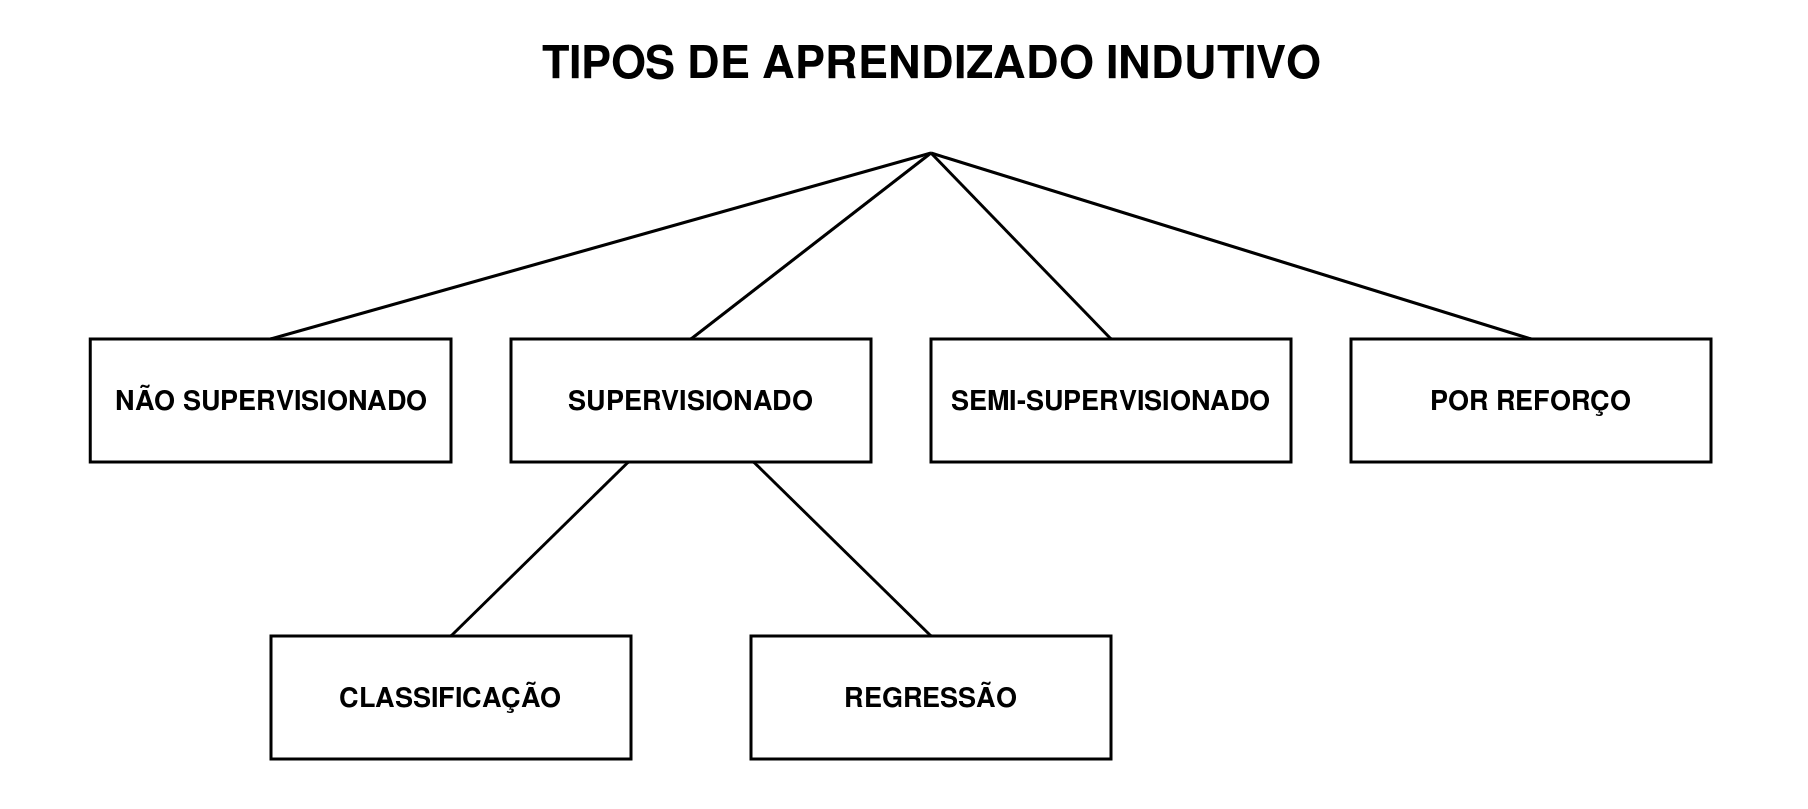
\includegraphics[width=1.0\textwidth]{{Cap2/tipos-aprendizado.png}}
\caption{Hierarquia dos tipos de aprendizado.}
\fonte{Fonte: \citeasnoun{lazarevic2005}}
\label{fig:tipos-aprendizado}
\end{figure}

No aprendizado supervisionado é necessário que os dados estejam rotulados, ou seja, apresentam qual o \textit{output} esperado pelo algoritmo. O \textit{output} é comumente chamado de rótulo ou classe. Desse modo, é possível definir um subconjunto de treinamento a ser utilizado para aquisição de conhecimento, enquanto outro subconjunto de testes é utilizado para cálculo de métricas de avaliação do modelo, como a acurácia, por exemplo. Quando os possíveis rótulos são valores finitos, o problema de aprendizado é chamado de classificação, podendo ser binária (dois possíveis valores), multi-classe (mais de dois valores possíveis) ou multi-rótulo (onde, independentemente do número de possíveis valores, existe a possibilidade de um único exemplo pertencer a mais de uma classe). Quando as possíveis classes existentes são valores contínuos, chama-se de regressão o problema de aprendizado.

O aprendizado não supervisionado, por sua vez, ocorre quando não há a presença dos rótulos, e é necessário que os algoritmos empregados no aprendizado sejam capazes de agrupar os exemplos contidos na base de dados somente analisando as características dos mesmos. Existe ainda o chamado semi-supervisionado, onde apenas parte das classes dos exemplos existentes são fornecidas. Dessa forma, os algoritmos tem o objetivo de buscar formas de, baseado nas observações com rótulo conhecido, aumentar o tamanho do conjunto rotulado, muitas vezes a fim de viabilizar o aprendizado supervisionado. Por fim, no aprendizado por reforço, o conhecimento é obtido por meio do resultado de decisões feitas pelo próprio sistema em processo de aprendizagem seguinte a estratégia de tentativa e erro. O resultado das decisões tomadas pode ocasionar recompensas boas ou ruins, e essa é a métrica utilizada para dimensionar o sucesso ou não da ação desempenhada pelo sistema.

O presente trabalho aborda a detecção de eventos intrusos e anômalos em ambiente computacional como um problema de classificação, manipulando a base de dados, de modo que possam ser avaliados dois cenários distintos: classificação binária e classificação multi-classe.

\subsection{Paradigmas}
\label{Sec:paradigmas}

As diversas abordagens e estratégias desenvolvidas ao longo dos anos na área de IA, mais especificamente na subárea de AM, podem ser classificadas de acordo com os paradigmas utilizados pelos algoritmos que as implementam. A seguir são apresentados alguns dos principais paradigmas aplicados em problemas de AM.

\subsubsection{Simbólico}

O paradigma simbólico, seguindo a ideia transmitida pela etimologia da palavra, remete a "sinais", "símbolos", "significados", e afins. Modelos construídos por meio de algoritmos que seguem este paradigma geralmente encontram-se representados na forma de expressões lógicas, árvores de decisão, regras ou redes semânticas \cite{maletzke2009}. Essas estruturas de modelos permitem a análise das regras inferidas nas etapas de treinamento, de modo que um especialista no domínio possa validar o aprendizado ocorrido.

\subsubsection{\textit{Instance-Based}}

Métodos deste gênero como, por exemplo, o algoritmo dos \emph{k} vizinhos mais próximos (K-\textit{Nearest Neighbors}), mantém o conjunto de exemplos de treinamento em memória, ao invés de criar um modelos que os represente. Deste modo, ao classificar um novo exemplo, métricas de distância ou similaridade são calculadas de modo a determinar quais observações, dentre as existentes na base de treinamento, possuem mais semelhanças com o novo elemento a ser classificado \cite{mitchell1997}. Embora ajam diversas vantagens em abordagens dessa natureza, a tarefa de classificação pode ser bastante custosa em comparação a outros mecanismos de classificação.

Poderia


\subsubsection{Genético}

Este paradigma está basicamente pautado na evolução simulada em ambiente computacional, com técnicas embasadas na definição de evolução da área de biologia. Algoritmos genéticos geralmente descrevem as hipóteses como sequências de \textit{bits}, e a interpretação dessas representações variam de acordo com o domínio de aplicação \cite{mitchell1997}. Desta forma, são definidas populações de exemplos iniciais, os quais são modificados de modo iterativo ao longo do que são as chamadas "gerações", mediante operações como reprodução ou mutação, dentre outras. A comparação entre indivíduos de diferentes populações é dada por uma função \textit{fitness}, a qual define uma métrica capaz de elencar os indivíduos mais bem adaptados.

\subsubsection{Conexionista}

O conexionismo, ou paradigma conexionista, é a área que estuda estruturas conhecidas como redes neurais artificiais. Essas estruturas também possuem inspiração biológica e buscam construir modelos mediante a extração de conhecimento implícito, contido nas relações existentes entre \textit{input} e \textit{output} \cite{rajagopalan1993}. Redes neurais artificiais serão abordadas com mais detalhes na seção seguinte.

\section{Redes Neurais Artificiais}

É estimado que o cérebro humano possua aproximadamente 10\textsuperscript{11} neurônios \cite{mitchell1997}, os quais tratam-se de células nervosas capazes de receber, processar e enviar informações. Os bilhares de neurônios também são capazes de conectar-se uns aos outros, possibilitando a construção do que é conhecido por rede neural. É através dessa complexa estrutura que os pulsos elétricos gerados por estímulos, externos ou do próprio corpo humano, são transmitidos e interpretados, possibilitando ao ser humano desempenhar tarefas complexas, como a tomada de decisão. \citeasnoun{haykin2001} define o cérebro como "um computador (sistema de processamento de informação) altamente complexo, não linear e paralelo".

Segundo o mesmo autor, uma das principais motivações para o desenvolvimento da área de redes neurais artificiais é a busca pela adaptação do uso de computadores convencionais, a fim de possibilitar aos mesmos desempenhar tarefas complexas, como reconhecimento de padrões e processamento visual. Por definição, uma rede neural artificial é "uma máquina projetada para modelar a maneira como o cérebro realiza uma tarefa particular ou função de interesse" \cite{haykin2001}.

A Figura \ref{fig:neuronio-biologico} apresenta a estrutura biológica dos neurônios, a qual é formada por corpo celular, dendritos, axônio e terminações do axônio, sendo que cada um possui papel fundamental no processo de recebimento de sinais elétricos e propagação dos mesmos ao longo de todo conglomerado de conexões neurais. A transmissão dos estímulos entre neurônios é denominada sinapse, e pode ser tanto excitatória, quanto inibitória aos chamados neurônios pós-sinápticos \cite{lent2004}.

\begin{figure}[H]
\centering 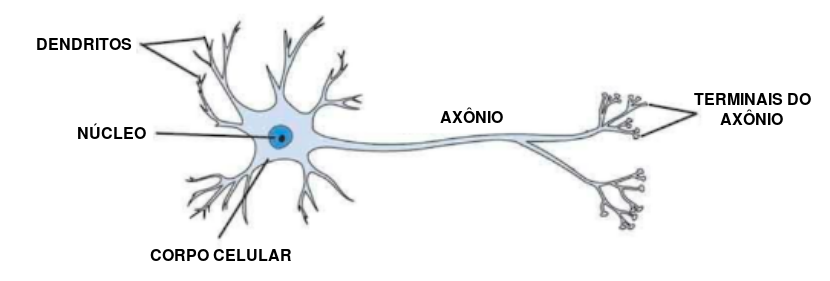
\includegraphics[width=\textwidth]{{Cap2/neuronio-biologico.png}}
\caption{Estrutura de um neurônio biológico.}
\fonte{Fonte: Adaptado de \citeasnoun{poel2019}.}
\label{fig:neuronio-biologico}
\end{figure}

Diante do exposto, para a construção de redes neurais artificiais são necessárias abstrações computacionais dos elementos que compõem a comunicação entre os neurônios, capazes de aprender mediante as interações ocorridas entre si, assim como acontece no cérebro humano. Na Figura \ref{fig:neuronio-artificial}, observa-se uma representação simplificada dessas abstrações. Alguns dos aspectos referentes a essa estrutura, que é comumente chamada de ``neurônio artificial``, serão abordadas nas seções seguintes.

\begin{figure}[H]
\centering 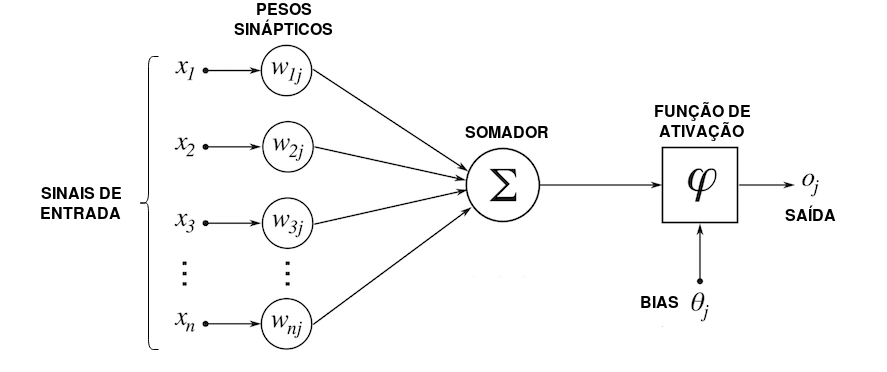
\includegraphics[width=\textwidth]{{Cap2/neuronio-artificial.png}}
\caption{Modelo matemático que representa um neurônio artificial.}
\fonte{Fonte: Adaptado de \citeasnoun{haykin2001}}
\label{fig:neuronio-artificial}
\end{figure}

\subsection{Funções de ativação}
\label{subsec:funcoes-ativacao}
Dentre os componentes do modelo matemático que representa o neurônio artificial cita-se a função da ativação. Cada um dos neurônios que compõem uma rede neural é capaz de guardar seu próprio estado interno, e o que determina esse estado é a função de ativação aplicada aos sinais de entrada, após multiplicados pelos ``pesos sinápticos`` e processados pelo ``somador``, conforme apresentado na Figura \ref{fig:neuronio-artificial}. O valor de saída da função de ativação de cada neurônio é então transmitido aos neurônios da próxima camada da rede que possuem conexão com o neurônio em questão.

Funções de ativação devem ser computacionalmente eficientes, dado que, dependendo da arquitetura da rede neural, as mesmas podem ser recalculadas milhões de vezes ao longo do treinamento do modelo neural. Diante disso, diferentes tipos de função de ativação foram propostos ao longo do tempo, geralmente tratando-se de funções matemáticas pouco complexas. Funções de ativação podem ser lineares ou não lineares, sendo que essas primeiras não possibilitam a aplicação do algoritmo \textit{backpropagation}, técnica amplamente utilizada no treinamento de redes neurais para estimar as derivadas necessárias para a definição dos gradientes no treinamento da RNA, possibilitando o ajuste dos pesos dos neurônios a fim de minimizar a perda de informação \cite{hecht1992}.

As funções de ativações não lineares de uso mais comum são apresentadas a seguir \cite{goodfellow2016}:
\begin{enumerate}
    \item \textbf{Sigmoide/Logística:} trata-se de uma função de ativação amplamente utilizada, pois apresenta comportamento balanceado entre linearidade e não-linearidade. Entretanto, características referentes às suas derivativas fazem com que atualmente seja desencorajado o uso das mesmas, com exceção de camadas de saída (para variáveis binárias) e casos específicos de redes recorrentes ou modelos probabilísticos, por exemplo \cite{goodfellow2016}. A saída dessa função é um valor contido no intervalo contínuo de 0 a 1. A função sigmoide é apresentada na Equação \ref{eq:sigmoide}. Na Figura \ref{fig:sigmoide} é possível observar o comportamento da função, tal como a sua derivada.
    \begin{equation}
    \label{eq:sigmoide}
        \sigma (x) ={1 \over 1 + e^{-x}}
    \end{equation}
    
    \begin{figure}[H]
        \centering 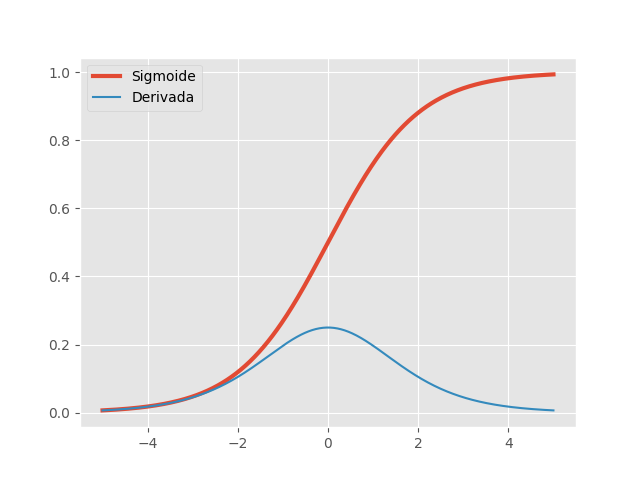
\includegraphics[width=0.90\textwidth]{{Cap2/sigmoide.png}}
        \caption{Gráfico da função de ativação Sigmoide.}
        \fonte{Fonte: \cite{facure2017}}
        \label{fig:sigmoide}
    \end{figure}
    
    \item \textbf{Tangente Hiperbólica (TanH):} bastante semelhante a função logística, porém com seu valor variando de -1 a 1, fazendo com que a parábola esteja centralizada no 0. A Equação \ref{eq:tanh} exibe a fórmula de cálculo da tangente hiperbólica. Na Figura \ref{fig:tanh}, que apresenta de forma gráfica o comportamento da função e de sua derivativa, é possível observar que o valor da derivada é maior quando comparada a função logística. Diante disso, quando é necessário o uso de uma função sigmoidal, geralmente utiliza-se a função \textit{tanh} \cite{goodfellow2016}.
    \begin{equation}
    \label{eq:tanh}
        tanh(x) = {2\sigma (2x) - 1}
    \end{equation}
    
    \begin{figure}[H]
        \centering 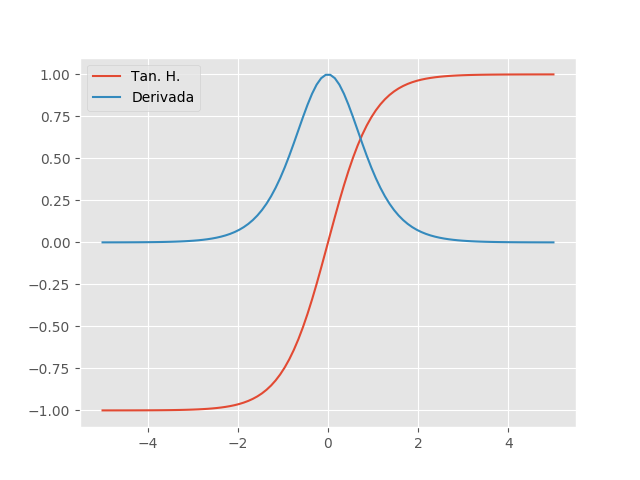
\includegraphics[width=0.90\textwidth]{{Cap2/tanh.png}}
        \caption{Gráfico da função de ativação Tangente Hiperbólica.}
        \fonte{Fonte: \cite{facure2017}}
        \label{fig:tanh}
    \end{figure}
    
    \item \textbf{Unidade Linear Retificada (ReLU):} conforme observado na Equação \ref{eq:relu}, trata-se de uma função praticamente linear, com exceção de metade do seu domínio (parte negativa), onde o valor de saída atribuído é zero. Desse modo, as derivativas mantém-se grandes (1, para valores positivos) e constantes, sendo possível também definir como 0 a derivada para valores negativos. Essa característica pode ser observada na Figura \ref{fig:relu}. Essa função de ativação demonstra ser extremamente poderosa diante da simplicidade unida a não linearidade.
    \begin{equation}
    \label{eq:relu}
        ReLU(x) = {max\{0,x\}}
    \end{equation}
    
    \begin{figure}[H]
        \centering 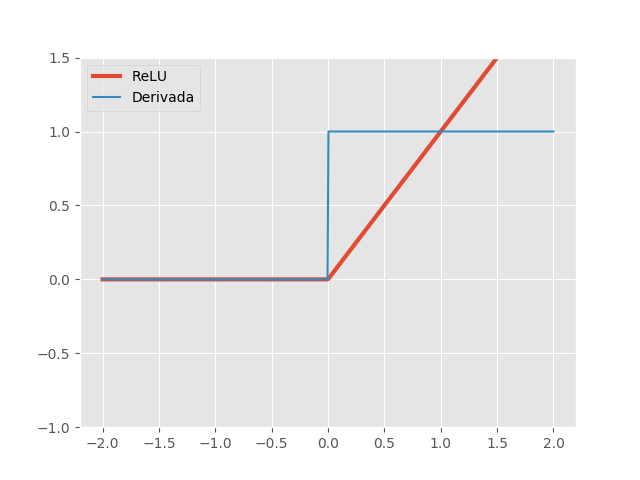
\includegraphics[width=0.90\textwidth]{{Cap2/relu.png}}
        \caption{Gráfico da função de ativação Unidade Linear Retificada.}
        \fonte{Fonte: \cite{facure2017}}
        \label{fig:relu}
    \end{figure}
    
    \item \textbf{Softmax:} outro tipo de função de ativação, geralmente utilizada na camada de saída, mas que também pode ser aplicada em camadas ocultas em casos específicos. Funções \textit{softmax} representam uma distribuição probabilística de uma variável discreta, apresentando uma probabilidade para cada valor possível \cite{goodfellow2016}. Ao contrário de funções sigmoide, a \textit{softmax} é capaz de trabalhar com problemas com mais de duas classes.

\end{enumerate}

\subsection{Treinamento}
\label{subsec:treinamento}
Conforme apresentado na Seção \ref{Sec:aprendizado}, existem diferentes paradigmas de aprendizado aplicados na construção de modelos de aprendizado de máquina. RNA realiza o aprendizado mediante um processo iterativo, onde os pesos sinápticos são reajustados, e isso é definido como a tarefa de treinamento da rede \cite{haykin2001}.

O processo de treinamento de RNA, como já mencionado, é realizado através da manipulação dos pesos atribuídos a cada um dos neurônios de entrada. Quando o treinamento é iniciado, esses pesos geralmente são inicializados de forma aleatória, fato que pode resultar em uma rede de baixa performance num primeiro momento, mas que pode convergir para uma rede com alta acurácia ao longos da iterações. Essas iterações são chamadas de épocas. A cada época de treinamento, os pesos são reajustados e então é realizado o treinamento novamente.

Diante disso, utiliza-se de uma função de perda para dar suporte ao reajuste dos pesos sinápticos. A função de perda, por sua vez, é uma das possíveis métricas que visam mensurar a performance de uma rede, onde redes com perda baixa apresentam resultados melhores do que aquelas que possuem perda alta. No aprendizado supervisionado, a perda é comumente calculada com base no erro do modelo, ou seja, a diferença entre os valores preditos e os valores reais dos exemplos da base de treino. Neste contexto, a tarefa de treinamento remete a um problema de otimização, no qual objetiva-se a minimização da perda da RNA.

Diferentes algoritmos de otimização foram propostos e empregados no treinamento de redes neurais ao longo do desenvolvimento da área de aprendizado de máquina. Um dos algoritmos mais simples é o \textit{Stochastic Gradient Descent} (SGD), o qual utiliza de gradientes, que por sua vez são vetores de derivativas, a fim de determinar se o ajuste de pesos da época atual deverá ser feito na direção positiva ou negativa, em busca do cenário ideal onde a perda é zero (0). Uma das limitações desse algoritmo é que um de seus parâmetros, a taxa de aprendizagem, é imutável ao longo do treinamento.

Para contornar esta limitação, outros algoritmos de otimização foram propostos como RMSProp (\textit{Root Mean Square Propagation}) e Adam (\textit{Adaptive Moment Estimation}). Ambos viabilizam uma taxa de aprendizagem dinâmica ao longo do treinamento da rede, embora o algoritmo Adam seja uma melhoria do RMSProp, e por isso têm sido mais utilizado em relação a outros algoritmos de otimização.

Desse modo, o treinamento de uma RNA se dá por meio da utilização de um algoritmo de otimização que busca minimizar a perda existente no modelo neural, sendo que a função de perda compreende em uma métrica para avaliar a performance da rede. O número de épocas pode ser previamente determinado de forma fixa, ou então depender de alguma condição definida na implementação da rede considerando o comportamento de alguns dos parâmetros da mesma, como, por exemplo, um critério de parada baseado em um limiar de perda ou de acurácia do modelo.

\subsection{Arquiteturas}
Outro aspecto essencial na definição de uma RNA é sua arquitetura, o que geralmente remete a sua estrutura, quantidade de neurônios e como os mesmos estão organizados e conectados \cite{goodfellow2016}. A maioria das RNA estão organizadas em sequenciais agrupamentos de neurônios (ou nós), chamados de camadas. Camadas de RNA podem ser de entrada, de saída ou ocultas. Os tipos básicos de camadas podem ser observados na Figura \ref{fig:arquitetura-basica}, onde a camada mais à esquerda corresponde a camada de entrada, a mais à direita corresponde a camada de saída, enquanto as demais são chamadas de camadas ocultas. Vale ressaltar que RNA podem possuir uma ou mais camadas ocultas, enquanto camadas de entrada e saída são únicas.

\begin{figure}[H]
        \centering 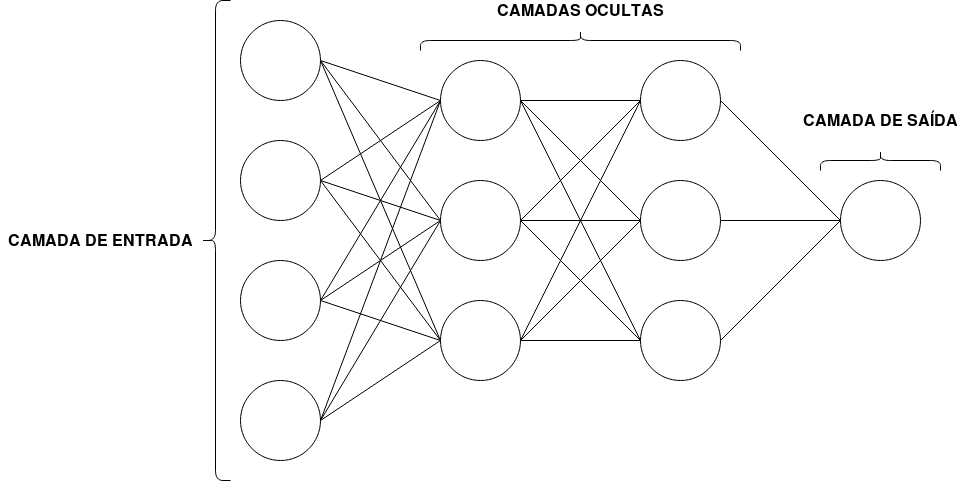
\includegraphics[width=\textwidth]{{Cap2/arquitetura-basica.png}}
        \caption{Arquitetura simplificada de uma rede neural com duas camadas ocultas.}
        \fonte{Fonte: Adaptado de \citeasnoun{datascienceacademy2019}.}
        \label{fig:arquitetura-basica}
    \end{figure}

A arquitetura disposta na Figura \ref{fig:arquitetura-basica} representa uma estrutura básica que a maioria das RNA seguem, embora possa haver diversas variações no \textit{design} das camadas ocultas, tanto em termos do número de camadas ocultas, quanto em relação ao número de neurônios existentes em cada uma dessas camadas. O \textit{design} dessas camadas intermediárias, ou ocultas, é ponto crucial na definição de um rede neural, principalmente de redes profundas, com mais de uma camada oculta. A área de que estuda redes mais profundas é denominada \textit{Deep Learning}.

No contexto deste trabalho serão abordadas redes nas quais as saídas das camadas são providas como entrada para as camadas posteriores \cite{haykin2001}. Tratam-se das chamadas redes neurais \textit{feedforward}. 
Dentre os diferentes tipos de redes \textit{feedforward}, a \textit{Multilayer Perceptron} (MLP) ganhou popularidade ao longo dos anos devido a sua capacidade de generalizar problemas não linearmente separáveis, o que é o caso de grande parte dos problemas reais existentes \cite{engelbrecht2007}.

Desse modo, com auxílio do algoritmo \textit{backpropagation} apresentado anteriormente, o treinamento se dá mediante propagação dos pesos sinápticos da camada de entrada para a camada de saída, passando por cada uma das camadas ocultas, sendo que nesse momento os pesos mantém-se inalterados. Após, com base no erro calculado utilizando-se do resultado esperado (aprendizado supervisionado) e do valor de saída da última camada, os pesos são ajustados e realiza-se uma nova iteração do treinamento. Considera-se que o treinamento foi concluído quando o erro for suficientemente pequeno. A partir disso, a rede passa a operar apenas em sentido \textit{forward} para a classificação de novos exemplos.

\subsection{Avaliação de Modelos}
\label{Sec:avaliacao-modelos}

Como apresentado previamente, os paradigmas e algoritmos empregados na solução de problemas de classificação são diversos, podendo inclusive serem utilizados de forma combinada e iterativa. De modo geral, no contexto de redes neurais, o produto do processo de treinamento constitui um modelo matemático capaz de realizar a classificação de novos exemplos, recebendo como \textit{input} valores referentes às \textit{features} do exemplo e retornando como \textit{output} o resultado da classificação desempenhada pela rede treinada.

A avaliação dos modelos construídos é imprescindível para examinar a viabilidade de aplicá-los em ambiente real. Diferentes estratégias são utilizadas com o objetivo de mensurar a capacidade de abstração dos modelos, visto que o principal objetivo de classificadores é a capacidade de generalização de problemas, a fim de obter bons resultados com exemplos não conhecidos e não pertencentes a base de treinamento.

Considerando o problema de classificação do presente trabalho no cenário binário, e \textit{N} e \textit{I} como sendo, respectivamente, o número de exemplos de eventos normais e intrusivos existentes na base de testes, é possível definir os seguintes termos:

\begin{itemize}
    \item \textit{True positive} (TP): compreende em exemplos positivos (ataques) classificados corretamente;
    \item \textit{False positive} (FP): elementos que foram apontados como ataque pelo classificador, mas que eram registros de atividade normal e genuína;
    \item \textit{True negative} (TN): exemplos de classe N classificados corretamente, ou seja, eventos normais detectados de forma apropriada;
    \item \textit{False negative} (FN): refere-se aos exemplos de classe negativa, ou seja, eventos intrusivos, classificados como eventos normais. Neste caso, trata-se do pior cenário possível, visto que um ataque computacional seria considerado como uma atividade normal.
\end{itemize}

Embora, neste trabalho, seja utilizada a nomenclatura supracitada, os termos dispostos são amplamente utilizados na literatura de forma traduzida, do seguinte modo: verdadeiro positivo, falso positivo, verdadeiro negativo e falso negativo. Além disso, vale ressaltar que esses termos não são exclusivos da área de detecção de intrusão e as relações entre classes positivas/negativas e eventos normais/intrusivos foram criadas apenas para facilitar o entendimento no contexto da área de aplicação em que se enquadra o presente trabalho.

Ao desempenhar o processo de teste de um modelo gerado, a partir de aprendizado supervisionado, é possível construir uma matriz de confusão. Matrizes de confusão consistem em tabelas que apresentam um resumo da classificação realizada pelo modelo, apontando o número de exemplos classificados em relação a classe predita e a verdadeira classe do elemento.

A matriz de confusão por si não é uma métrica de avaliação de modelos de classificação, porém, diversas análises e métricas podem ser feitas a partir de tais informações. Na Tabela \ref{tab:matriz-confusao} é possível observar um exemplo de matriz de confusão.

\begin{table}[H]
    \centering
    \begin{tabular}{c||cc}
        \hline
        \textbf{Classe} & \multicolumn{2}{c}{\textbf{Classe Predita}} \\
        \hline
        \hline
        & Ataque (+) & Normal (-) \\
        Ataque (+) & TP & FP \\
        Normal (-) & FN & TN \\
        \hline
    \end{tabular}
    \caption{Exemplo de uma matriz de confusão}
    \fonte{Fonte: O autor.}
    \label{tab:matriz-confusao}
\end{table}

Conforme mencionado, com base nos termos que descrevem o processo de classificação apresentados, é possível o cálculo de diferentes métricas que auxiliam a avaliação dos modelos classificadores construídos por algoritmos de AM. Algumas dessa métricas são apresentadas a seguir:

\begin{enumerate}
    \item \textbf{Acurácia:} esta métrica é responsável pelo cálculo da proporção de exemplos corretamente classificados em relação ao total de exemplos existentes no subconjunto de testes. Em casos de acentuado desbalanceamento de classes, pode não ser um bom aspecto a ser considerado. A acurácia é calculada a partir da Equação \ref{eq:acuracia}, apresentada a seguir:
        
        \begin{equation} \label{eq:acuracia}
        \frac{TP + TN}{TP + TN + FP + FN}
        \end{equation}
        
    \item \textbf{Precisão:} estima a proporção de exemplos classificados como ataques em relação ao total de exemplos que de fato são pertencentes a esta classe. A fórmula para o cálculo da precisão pode ser visualizada na Equação \ref{eq:precisao}:
        
        \begin{equation} \label{eq:precisao}
        \frac{TP}{TP + FP}
        \end{equation}
        
    \item \textbf{\textit{Recall} ou \textit{True Positive Rate} (TPR):} também conhecida como sensibilidade, esta medida é calculada a fim de estimar a proporção entre exemplos que efetivamente são eventos intrusivos e aqueles que foram classificados como tal pelo algoritmo. A Equação \ref{eq:recall} demonstra como é calculada a sensibilidade de um modelo:
        
        \begin{equation} \label{eq:recall}
        \frac{TP}{TP + FN}
        \end{equation}
    
    \item \textbf{F1-Score:} trata-se de uma métrica que relaciona precisão e \textit{recall} através de uma média harmônica, atribuindo maior peso para o menor dos valores. O cálculo é realizado conforme apresentado na Equação \ref{eq:f1-score}:

        \begin{equation} \label{eq:f1-score}
        2 \times \frac{PR \times RE}{PR + RE}
        \end{equation}
        
        onde~$PR$ corresponde ao cálculo de precisão e~$RE$ ao cálculo de \textit{recall}.
\end{enumerate}

Diante do exposto, é possível observar a seguinte relação entre as métricas apresentadas e a performance do modelo construído:

\begin{itemize}
    \item \textbf{Alto \textit{recall} e alta precisão:} a classe é perfeitamente classificada pelo modelo.
    \item \textbf{Baixo \textit{recall} e alta precisão:} o modelo não é capaz de classificar a classe tão bem, porém é bastante confiável quando o faz.
    \item \textbf{Alto \textit{recall} e baixa precisão:} a classe é detectada de forma muito boa, mas o modelo também relaciona exemplos de outras classe a este rótulo.
    \item \textbf{Baixo \textit{recall} e baixa precisão:} o modelo não é capaz de classificar exemplos pertencentes a esta classe de forma satisfatória.
\end{itemize}

\section{Bases de Dados}
\label{Sec:bases}

Existem diferentes formas de obter informações sobre tráfego de dados em ambiente computacional, como captura de pacotes, registro de \textit{logs}, dentre outros. Estas podem ser de grande valia quando empregadas na identificação de eventos anômalos ocorridos. No intuito de fornecer tais informações para construção de modelos classificadores, é imprescindível que esses registros estejam devidamente representados e organizados, pois somente desta forma torna-se viável o processamento dos dados mediante várias das técnicas existentes na subárea de AM.

Bases de dados de detecção de intrusão, os chamados \textit{datasets}, são coleções de eventos de rede disponibilizados por diferentes organizações, sendo que, eventualmente, os registros desses eventos são rotulados de acordo com o tipo de evento que se trata (normal ou ataque). 

Após o surgimento das primeiras bases de dados com eventos de rede rotulados, como DARPA 98 e KDD Cup 99, outros grupos também despenderam de esforços para a construção de novas bases. Por se tratar de dados críticos, e que caso não sejam devidamente tratados e preprocessados, podem eventualmente expôr detalhes confidenciais e sigilosos, muitas das organizações que desenvolvem pesquisa nessa área preferem não tornar públicos os dados capturados e utilizados. Esse e outros fatores contribuíram para a utilização de bases desatualizadas como balizadoras de métodos de detecção de intrusão até os tempos atuais.

Em contrapartida, existem também grupos de pesquisa que presam pelo compartilhamento dos eventos capturados e pela criação de bases de dados públicas, com eventos relacionados a fluxo de redes de computadores. Vale ressaltar a grande complexidade envolvida na criação de bases desse gênero, abrangendo desde a estruturação de ambiente computacional complexo, que represente infraestruturas utilizadas em cenários reais, até a simulação de diferentes tipos de ataques computacionais modernos e organização dos eventos capturados.

Na sequência dessa seção serão abordadas, de forma sucinta, as principais características de algumas das bases de dados públicas mais aplicadas na avaliação de sistemas de detecção de intrusão.

\subsection{DARPA / KDD Cup 99}
\label{Subsec:kdd99}

No ano de 1998 foi criada, no Instituto de Tecnologia de Massachusetts (MIT), mais especificamente no "Lincoln Laboratory", a primeira base de dados pública contendo registros de eventos capturados em redes de computadores, para avaliação de sistema de detecção de intrusão. Um dos patrocinadores do projeto foi a agência de pesquisa de defesa americana, DARPA, justificando a escolha do nome: DARPA 1998\footnote{https://www.ll.mit.edu/r-d/datasets/1998-darpa-intrusion-detection-evaluation-dataset}. Foi concebida com o intuito de auxiliar pesquisadores que desenvolvem a área de detecção de intrusão, principalmente pelo fato de servir como fator balizador e grupo controle para realização de comparações consistentes.

No ano seguinte, após ajustes na dinâmica da geração dos fluxos de rede para captura, foi criada a nova versão da base de dados, DARPA 1999\footnote{https://www.ll.mit.edu/r-d/datasets/1999-darpa-intrusion-detection-evaluation-dataset}. Para a construção desta base foram utilizados tráfegos de dados simulados e reais \cite{thomas2008}. Todo o tráfego de rede foi capturado e armazenado mediante a ferramenta \textit{tcpdump}\footnote{https://www.tcpdump.org/}, ao longo de nove semanas de experimentos. Os pacotes de rede compreendem atividades normais e eventos gerados a partir de diferentes classes de ataques, sendo que os ataques desempenhados podem ser agrupados em quatro diferentes categorias: \textit{Denial of Service} (DoS), \textit{Probe}, R2L (\textit{Remote to Local}) e U2R (\textit{User to Root}).

Devido ao fato do formato gerado pela ferramenta \textit{tcpdump} não ser compatível com a maioria dos algoritmos de aprendizado de máquina, foi desenvolvida a base KDD Cup 99\footnote{http://kdd.ics.uci.edu/databases/kddcup99/kddcup99.html}, a fim de ser utilizada na tradicional competição "KDD Cup", a qual trata-se de um concurso na área de descoberta de conhecimento em bases de dados com temáticas variadas ao longo dos anos. A KDD Cup 99 é composta por 41 \textit{features} extraídas dos pacotes de rede existentes na DARPA 1998, abrangendo tanto características básicas obtidas diretamente dos pacotes, como protocolo, portas e \textit{flags}, quanto dados de conteúdo dos pacotes, medidas estatísticas e atributos baseados em tempo \cite{liu2019}. Os exemplos são rotulados de acordo com as mesmas classes de ataques, além do comportamento normal, totalizando cinco diferentes possíveis valores para o atributo de classe.

Ao longo dos anos esta base foi amplamente aplicada no desenvolvimento de SDI. Apesar da enorme popularidade, estudos posteriores apontaram limitações e deficiências existentes na mesma. Primeiramente cita-se o enorme desbalanceamento dos dados, fazendo com que os modelos classificadores fossem enviesados para a classe majoritária. Além disso, o grande número de duplicata de dados, informações redundantes \cite{mchugh2000}, necessidade de preprocessamento, muitas vezes feito de forma não padronizada entre os trabalhos, e a pouca representatividade de eventos atuais, fez com que várias críticas surgissem quanto a utilização desse conjunto de dados \cite{liu2019}.

\subsection{CAIDA}

O conjunto de dados CAIDA \cite{caida2007} é composto por aproximadamente uma hora de tráfego de dados, correspondente a um ataque de distribuído de negação de serviço, ou DDoS. A base é composta por diversos arquivos no formato \textit{.pcap}, totalizando em 5.3 GB quando compactados (21 GB descompactados). Esse volume de dados ilustra o poder que ataques dessa natureza possuem, visto que todo esse tráfego foi gerado de forma distribuída, focando em um único alvo a fim de ocupar todos os recursos disponíveis no servidor vítima.

O formato em que os dados são disponibilizados torna necessário o tratamento dos mesmos antes que possam ser submetidos a algoritmos de aprendizado de máquina, como comentado previamente. Além disso, pode-se citar como desvantagem dessa base a não existência de uma diversidade de ataques, nem de pacotes referentes a atividades consideradas normais \cite{khraisat2019}.

\subsection{NSL KDD}

Como já mencionado, diversos trabalhos realizam críticas e apresentam desvantagens e limitações da base KDD Cup 99 \cite{mchugh2000, wang2014}. Em \citeasnoun{tavallaee2009}, além de apresentar aspectos negativos desta base, os autores propuseram soluções para a maioria dos problemas que julgaram necessários, resultando na construção de um novo conjunto de dados, com base na KDD Cup 99.

Essa nova base denomina-se NSL-KDD e apresenta os mesmos atributos existentes em sua base de origem, porém com número de exemplos significativamente diminuído. Enquanto a KDD Cup 99, em sua versão completa, possui mais de quatro milhões de exemplos, a NSL-KDD possui apenas 125.973, o que possibilita a execução de treinamento de modelos complexos utilizando o conjunto de dados completo ao invés de utilizar apenas amostras menores e aleatórias.

Embora diversas particularidades, como as levantadas por \citeasnoun{mchugh2000}, tenham sido corrigidas por \citeasnoun{tavallaee2009} e pesquisadores ainda acreditem que este conjunto de dados podem ser considerado um \textit{benchmark} relevante para comparar diferentes métodos de detecção de intrusão, a NSL-KDD ainda possui deficiências, principalmente no que se refere ao pequeno número de exemplos para determinadas classes de ataques e a representatividade de eventos de rede atuais, visto que os exemplos em si reflete a infraestruturas e eventos do ano de 1999.

\subsection{ISCX 2012}

A base de dados ISCX 2012 foi construída a partir de dados capturados em 2010, ao longo de uma semana, incluindo atividade normal e ataques de infiltração, negação de serviço (DoS), negação de serviço distribuído e força bruta SSH\footnote{\label{fn:iscx2012}https://www.unb.ca/cic/datasets/ids.html}. O processo de construção desta base, por sua vez, seguiu uma abordagem sistemática, definida em \citeasnoun{shiravi2012}, que contém uma arquitetura complexa desenvolvida em laboratório e que envolve dezenas de \textit{workstations} Windows e servidores Web (Linux e Windows), provendo serviços de e-mail, DNS (\textit{Domain Name System}) e NAT (\textit{Network Address Translation}) \cite{fernandez2019}. A arquitetura da rede de experimentação utilizada para a construção da base ISCX2012 pode ser observada na Figura \ref{fig:arquitetura-iscx}.

\begin{figure}[H]
    \centering 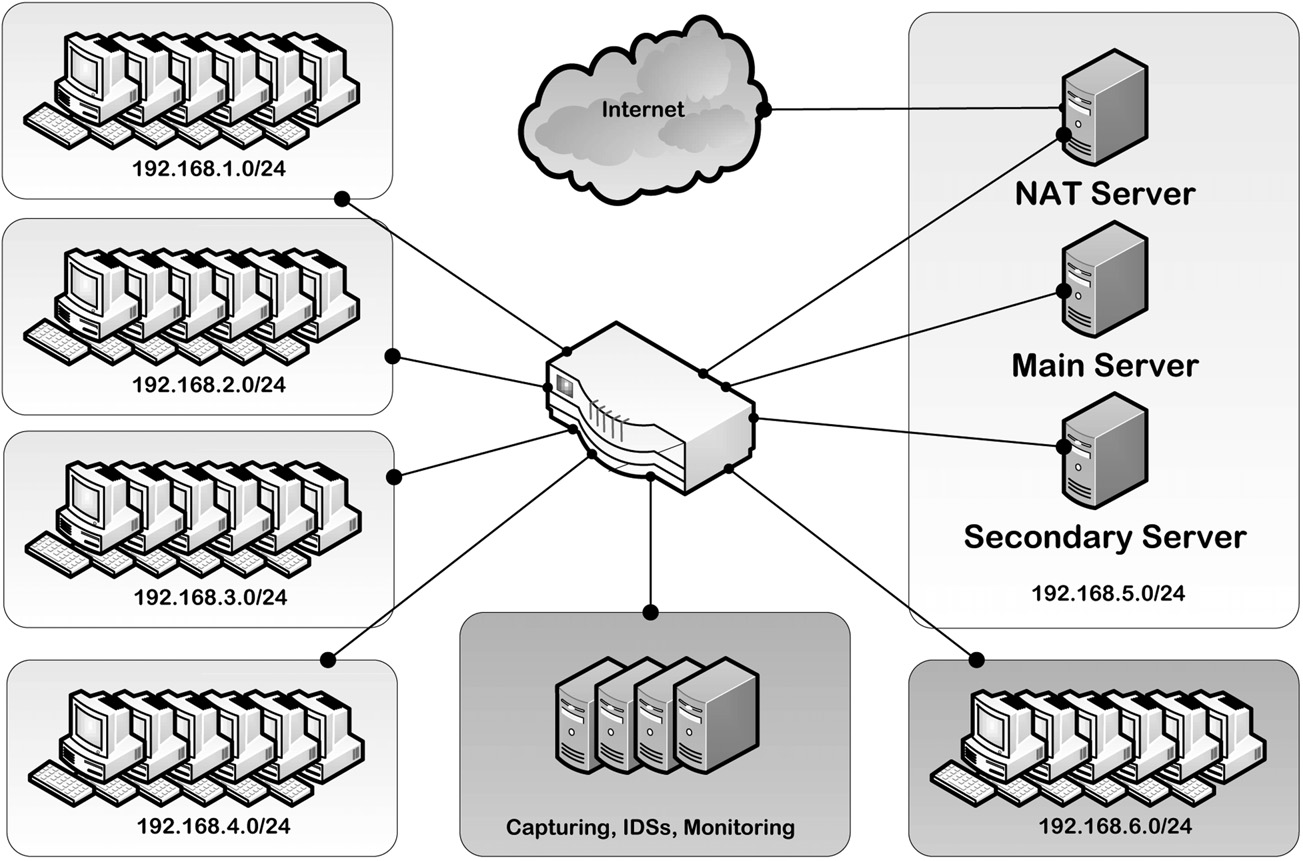
\includegraphics[width=\textwidth]{{Cap2/arquitetura-iscx.png}}
    \caption{Arquitetura da Rede de Experimentação utilizada na construção da base ISCX 2012. Fonte: \cite{shiravi2012}.}
    \label{fig:arquitetura-iscx}
\end{figure}

Algumas das características da ISCX 2012 são \footnoteref{fn:iscx2012} \cite{shiravi2012}: ambiente de rede realístico; tráfego realístico; dados rotulados em tráfego benigno ou malicioso; captura total das interações entre os envolvidos nas comunicações; e diversos cenários de ataques distintos. A base completa apresenta mais de dois milhões e meio de registros de fluxos de dados, sendo que apenas 68.910 (aproximadamente 2,71\%) correspondem a eventos intrusivos.

\citeasnoun{gharib2016} definem um \textit{framework} de avaliação de SDI, sugerindo qualidades necessárias para a construção de um bom conjunto de dados. As características da ISCX 2012 mencionadas englobam grande parte do que foi definido por \citeasnoun{gharib2016}. Embora demonstre ser uma boa opção para avaliação de sistemas de detecção de intrusão, a existência de bases mais atuais desmotivou a utilização da ISCX 2012 no contexto deste trabalho.

\subsection{CICIDS 2017}
\label{Subsec:cicids2017}

Assim como as bases NSL-KDD e ISCX 2012, anteriormente citadas, a CICIDS 2017 é fruto de trabalhos desenvolvidos pelo grupo de pesquisa \textit{Canadian Institute of Cybersecurity}, da Universidade de New Brunswick, Canadá e seus parceiros\footnote{http://www.unb.ca/cic/datasets/ids-2017.html}.

Este conjunto de dados foi construído a partir da captura de tráfego de rede durante cinco dias (de segunda a sexta), onde o primeiro dia foi o único sem ataques. Ao longo dos dias seguintes foram realizados ataques de força bruta FTP e SSH, DoS e DDoS, \textit{Heartbleed}, ataques Web, infiltração e \textit{Botnet}. Na Tabela \ref{tab:ataques_cicids2017} estão contidos todos os ataques desempenhados na construção da base, onde é possível observar que a diversidade de ataques é maior quando comparada a ISCX 2012.

\begin{table}[H]
    \centering
    \begin{tabular}{cc}
        \hline
        \multicolumn{2}{c}{\textbf{Tipos de Ataques}} \\
        \hline
        Bot & Heartbleed \\
        DDoS & Infiltration \\
        DoS GoldenEye & PortScan \\
        DoS Hulk & SSH-Patator \\
        DoS Slowhttptest & Web Attack \textbackslash x96 Brute Force \\
        DoS Slowloris & Web Attack \textbackslash x96 Sql Injection \\
        FTP-Patator & Web Attack \textbackslash x96 XSS \\
        \hline
    \end{tabular}
    \caption{Tipos de ataques computacionais desempenhados na construção da base de dados CICIDS 2017.}
    \label{tab:ataques_cicids2017}
    \fonte{Fonte: O autor.}
\end{table}


Um dos pontos relevantes da construção dessa base é que no estabelecimento da arquitetura, da rede vítima, foram levados em conta todos os equipamentos comumente necessários no cenário real, como roteadores, \textit{firewall}, \textit{switches} e os três (3) principais sistemas operacionais: Windows, Linux e Macintosh. A arquitetura completa é exposta na Figura \ref{fig:arquitetura-cic}, enquanto os demais detalhes da construção da base podem ser vistos em \citeasnoun{sharafaldin2018}.

\begin{figure}[H]
    \centering 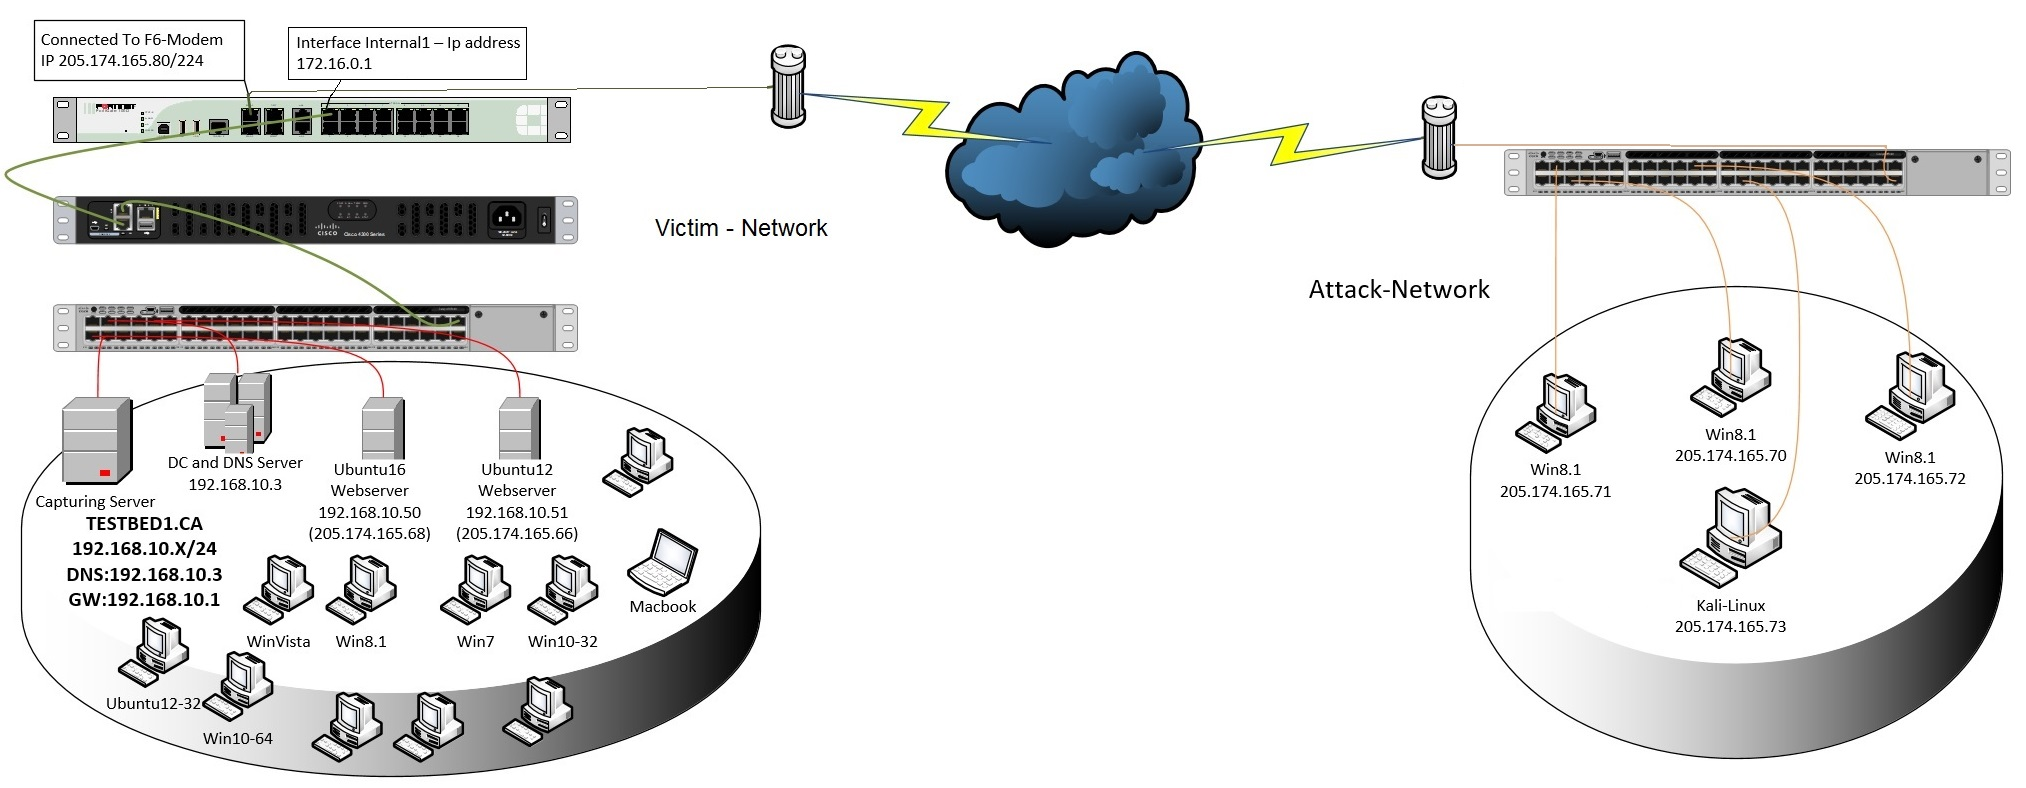
\includegraphics[width=\textwidth]{{Cap2/arquitetura-cic.png}}
    \caption{Arquitetura de rede utilizada na construção da base CICIDS 2017.}
    \label{fig:arquitetura-cic}
    \fonte{Fonte: \cite{sharafaldin2018}.}
\end{figure}

Os dados brutos são providos em formato \textit{pcap}, sendo que o tamanho dos arquivos referentes a cada dia de experimento encontra-se na faixa dos \textit{gigabytes}, o que demonstra o alto volume de tráfego gerado e capturado na concepção dessa base.

Além dos dados brutos capturados durante as simulações desempenhadas, os registros também são fornecidos de modo rotulado, classificados de acordo com a natureza das conexões: normal ou invasiva. A representação atributo-valor dos dados rotulados são disponibilizado em formato \textit{csv}, sendo que esta estruturação foi viabilizada pela ferramenta CICFlowMeter\footnote{http://netflowmeter.ca/} (também conhecida como ISCXFlowMeter). Trata-se de um extrator de atributos de fluxo de dados que pode atuar como \textit{sniffer}, extraindo os atributos do tráfego de uma \textit{interface} de rede em tempo real, ou processar arquivos em formato \textit{pcap}, realizando a extração dos atributos após a captura dos pacotes (\textit{offline}).

Atualmente o CICFlowMeter permite a extração de mais de 150 atributos\footnote{http://www.netflowmeter.ca/netflowmeter.html}. Quando a base de dados CICIDS 2017 foi concebida, foram extraídos 84 atributos, os quais são dispostos a seguir:

\begin{longtable}{r|p{10.5cm}}
\hline
\centering
    \textbf{Atributo}  & \textbf{Descrição}   \\
    \hline
    Flow.ID & Identificador do fluxo \\
    Source.IP & IP origem \\
    Source.Port & Porta origem \\
    Destination.IP & IP destino \\
    Destination.Port & Porta destino \\
    Protocol & Tipo do protocolo do fluxo \\
    Timestamp & Data e hora do início do fluxo \\
    Flow.Duration & Duração do fluxo em milissegundos \\
    Total.Fwd.Packets & Total de pacotes \textit{forward} \\
    Total.backward.Packets & Total de pacotes \textit{backward} \\
    Total.Length.of.Fwd.Packets & Tamanho total dos pacotes \textit{forward} \\
    Total.Length.of.Bwd.Packets & Tamanho total dos pacotes \textit{backward} \\
    Fwd.Packet.Length.Max & Tamanho do maior pacote \textit{forward} \\
    Fwd.Packet.Length.Min & Tamanho do menor pacote \textit{forward} \\
    Fwd.Packet.Length.Mean & Média de tamanho dos pacotes \textit{forward} \\
    Fwd.Packet.Length.Std & Desvio padrão do tamanho dos pacotes no sentido \textit{forward} \\
    Bwd.Packet.Length.Max & Tamanho do maior pacote \textit{backward} \\
    Bwd.Packet.Length.Min & Tamanho do menor pacote \textit{backward} \\
    Bwd.Packet.Length.Mean & Média de tamanho dos pacotes \textit{backward} \\
    Bwd.Packet.Length.Std & Desvio padrão do tamanho dos pacotes no sentido \textit{backward} \\
    Flow.Bytes.s & Número de \textit{bytes} por segundo no fluxo \\
    Flow.Packets.s & Número de pacotes por segundo no fluxo \\
    Flow.IAT.Mean & Média do IAT no fluxo \\
    Flow.IAT.Std & Desvio padrão do IAT de todos os pacotes do fluxo \\
    Flow.IAT.Max & Valor do maior IAT do fluxo \\
    Flow.IAT.Min & Valor do menor IAT do fluxo \\
    Fwd.IAT.Total & IAT total sentido \textit{forward} \\
    Fwd.IAT.Mean & Média do IAT no sentido \textit{forward} \\
    Fwd.IAT.Std & Desvio padrão do IAT de todos os pacotes do fluxo \\
    Fwd.IAT.Max & Maior valor de IAT no sentido \textit{forward} \\
    Fwd.IAT.Min & Menor valor de IAT no sentido \textit{forward} \\
    Bwd.IAT.Total & IAT total no sentido \textit{backward} \\
    Bwd.IAT.Mean & Média do IAT no sentido \textit{backward} \\
    Bwd.IAT.Std & Desvio padrão do IAT dos pacotes \textit{backward} \\
    Bwd.IAT.Max & Maior valor de IAT no sentido \textit{backward} \\
    Bwd.IAT.Min & Menor valor de IAT no sentido \textit{backward} \\
    Fwd.PSH.Flags & Contador da \textit{flag} PSH em pacotes no sentido \textit{forward} \\
    Bwd.PSH.Flags & Contador da \textit{flag} PSH em pacotes no sentido \textit{backward} \\
    Fwd.URG.Flags & Contador da \textit{flag} URG em pacotes no sentido \textit{forward} \\
    Bwd.URG.Flags & Contador da \textit{flag} URG em pacotes no sentido \textit{backward} \\
    Fwd.Header.Length & Total de \textit{bytes} usados para o \textit{header} no sentido \textit{forward} \\
    Bwd.Header.Length & Total de \textit{bytes} usados para o \textit{header} no sentido \textit{backward} \\
    Fwd.Packets.s & Número de pacotes por segundo no sentido \textit{forward} \\
    Bwd.Packets.s & Número de pacotes por segundo no sentido \textit{backward} \\
    Min.Packet.Length & Tamanho do menor pacote \\
    Max.Packet.Length & Tamanho do maior pacote \\
    Packet.Length.Mean & Média dos tamanhos dos pacotes no fluxo \\
    Packet.Length.Std & Desvio padrão dos tamanhos dos pacotes no fluxo \\
    Packet.Length.Variance & Variância dos tamanhos dos pacotes no fluxo \\
    FIN.Flag.Count & Contador da \textit{flag} FIN nos pacotes do fluxo \\
    SYN.Flag.Count & Contador da \textit{flag} SYN nos pacotes do fluxo \\
    RST.Flag.Count & Contador da \textit{flag} RST nos pacotes do fluxo \\
    PSH.Flag.Count & Contador da \textit{flag} PSH nos pacotes do fluxo \\
    ACK.Flag.Count & Contador da \textit{flag} ACK nos pacotes do fluxo \\
    URG.Flag.Count & Contador da \textit{flag} URG nos pacotes do fluxo \\
    CWR.Flag.Count & Contador da \textit{flag} CWR nos pacotes do fluxo \\
    ECE.Flag.Count & Contador da \textit{flag} ECE nos pacotes do fluxo \\
    Down.Up.Ratio & Proporção entre \textit{download} a \textit{upload} \\
    Average.Packet.Size & Média do tamanho dos pacotes \\
    Avg.Fwd.Segment.Size & Média de tamanho de segmentos no sentido \textit{forward} \\
    Avg.Bwd.Segment.Size & Média de tamanho de segmentos no sentido \textit{backward} \\
    Fwd.Avg.Bytes.Bulk & Média de \textit{bytes} de transmissão em massa no sentido \textit{forward} \\
    Fwd.Avg.Packets.Bulk & Média de pacotes de transmissão em massa no sentido \textit{forward} \\
    Fwd.Avg.Bulk.Rate & Média de taxa de transmissão em massa no sentido \textit{forward} \\
    Bwd.Avg.Bytes.Bulk & Média de \textit{bytes} de transmissão em massa no sentido \textit{backward} \\
    Bwd.Avg.Packets.Bulk & Média de pacotes de transmissão em massa no sentido \textit{backward} \\
    Bwd.Avg.Bulk.Rate & Média de taxa de transmissão em massa no sentido \textit{backward} \\
    Subflow.Fwd.Packets & Número de pacotes em um \textit{subflow} no sentido \textit{forward} \\
    Subflow.Fwd.Bytes & Número de \textit{bytes} em um \textit{subflow} no sentido \textit{forward} \\
    Subflow.Bwd.Packets & Número de pacotes em um \textit{subflow} no sentido \textit{backward} \\
    Subflow.Bwd.Bytes & Número de \textit{bytes} em um \textit{subflow} no sentido \textit{backward} \\
    Init\_Win\_bytes\_forward & Total de \textit{bytes} enviados na janela inicial no sentido \textit{forward} \\
    Init\_Win\_bytes\_backward & Total de \textit{bytes} enviados na janela inicial no sentido \textit{backward} \\
    Act\_Data\_Pkt\_Fwd & Pacotes com ao menos 1 byte de \textit{payload} no sentido \textit{forward} \\
    Min\_Seg\_Size\_Forward & Tamanho mínimo de segmento observado no sentido \textit{forward} \\
    Active.Mean & Tempo médio de atividade dos fluxos \\
    Active.Std & Devio padrão do tempo de atividade dos fluxos \\
    Active.Max & Tempo máximo de atividade dos fluxos \\
    Active.Min & Tempo mínimo de atividade dos fluxos \\
    Idle.Mean & Tempo médio de ociosidade dos fluxos \\
    Idle.Std & Devio padrão do tempo de ociosidade dos fluxos \\
    Idle.Max & Tempo máximo de ociosidade dos fluxos \\
    Idle.Min & Tempo mínimo de ociosidade dos fluxos \\
    Label & Rótulo \\
    \hline
    \caption{Descrição dos atributos existentes na base CICIDS 2017.\newline Fonte: O autor.}
    \label{tab:atributos-cic}
\end{longtable}